\chapter{Transformation-based Error-driven Learning in Dependency Parsing}

\section{Introduction}
\label{sc:main}

Dependency parsing results tend to be reliable as long as the parser is trained and tested on data from a single domain. However, the situation is considerably more challenging when the data set on which the parser is tested/used is different from the sentences on which it is trained. For example, a parser trained on newspaper corpus would not parse texts based on spontaneous dialogues accurately. Since it is impossible to manually annotate the amount of data needed to train a parser in any domain that we need to parse, we need automatic methods to adapt a parser to those new domains. %Manual annotation is even harder when the syntactic structure of the data differs widely. E.g., the syntactic structure of a newspaper corpus is very different from that of natural language dialogue corpus or literary works. This leads to significant differences in the way these corpora are annotated to capture these inherent differences. 
%%SK: that is not true, theoretically, you can use the same scheme, but practically there are phenomena in the target domain that are important, but you definitely cannot introduce this as an integral part of domain adaptation.
This problem is generally addressed in domain adaptation. Domain adaptation attempts to use a large set of annotated data from a different domain plus specific strategies to adapt the annotations to the target domain, for which a small amount of annotated data may exist. The problem is compounded when there are differences in the annotation schemes between the source and target domain. Different treebanks, representing different domains, tend to  use somewhat different annotations \cite{dredze2007frustratingly}. These differences can be due to individual syntactic interpretations of different annotators, but in many cases, they are necessitated by phenomena in the target domain that do not exist in the source domain. Spontaneous dialogues, for example, have a large number of incomplete sentences with words that cannot be attached easily if their head is missing (e.g., the determiner in ``I bought the -'').
%This is because the parser learns the syntactic constructions from the source domain corpus, i.e., the newspaper corpus in this case, which does not always apply to the target corpus, the dialogue corpus. Hence, these differences leads to incorrect structural as well as functional errors or both. Structural errors affect the structure of a parse tree, i.e., when the head of a dependency arc is predicted incorrectly affecting the unlabeled attachment scores. Inaccurate prediction of the label of the arc results in functional errors. This lowers the labeled attachment scores as well as label accuracy. 

Out-of-domain dependency parsing results tend to be low as compared to in-domain results. The problem can be looked at from different perspectives. Previous work in this area has extensively looked at the structural errors, where the dependency arcs are corrected. For instance, the DeSR parser~\cite{attardi2007multilingual, attardi2007tree, attardi2009accurate} implements tree revisions. %, i.e., the mistakes made by the base parser for the target domain are rectified by the tree revision method. I.e., the change is at a structural level where the dependency arcs are moved to a different head in the dependency tree. 
Structural change of dependency trees prove to be an effective domain adaptation method. %The method improves the unlabeled attachment scores (UAS). 
\citet{yu2015domain} report a 1.6\% improvement by using self-training to generate training examples for the target domain. To our knowledge, no methods have been reported addressing functional errors, i.e., errors in the dependency labels.

Our work focuses on a target domain of spontaneous dialogues, using the CReST Corpus \citep{eberhard2010indiana}, %Here, the situation is complicated by the fact that 
which uses labels that do not occur in the source domain corpus. We propose to use 
%apply a method which could reduce structural as well as functional errors. In this paper, we look at functional errors. Functional errors originating from the difference in dependency labels between source and the target domain contributes to a significant reduction in the labeled attachment scores. This is evident when the source and target domains have different number of dependency labels. E.g., the target domain could have a subset of source domain labels. In that case, a parser trained on source domain would parse a sentence from target domain differently leading to a drop in LAS. The problem is equally challenging for the other scenario, where source has a subset of target labels. In that case, the parser has not seen the labels in the source and it will almost certainly parse it wrong. 
transformation based error driven learning (TBL) \cite{Brill:1995:TEL:218355.218367} to address the problem. The method has been proven effective in a variety of NLP problems including POS tagging and syntactic parsing. The idea is simple:  We use a small annotated data set in the target domain and automatically annotate it using a source domain parser.  Our goal to learn a set of rules from the errors that occur and a set of rule templates. 
%We emulate this approach with modifications to learn rules by applying transformations to a text annotate by a parser trained on a different domain. Our method rectifies the errors in dependency labels even in the case where a particular label doesn't appear in source. Thus, it greatly improves the labeled attachment score. The main advantages of this method are - it only requires a small amount data for training and it is easily generalizable for any domain. 
Although we focus on correcting dependency labels in the current paper, our method can be extended to correct the errors in dependency arcs as well.
%In this paper, 
We demonstrate that using TBL with a small target domain training set improves dependency parsing accuracy by about 10 \% absolute, and it learns to use the target-specific labels. 

The paper is structured as follows: Section~\ref{sec:related} discusses related work, section~\ref{sec:background} describes the issues in domain adaptation in more detail, and section~\ref{sec:tbl} explains our approach of using
TBL for domain adaptation. In section~\ref{sec:exptsetup}, we describe our experiment setup, and section~\ref{expt_results} discusses the results. Section~\ref{conclusion} concludes and delineates
future work.


\section{Related Work} \label{sec:related}

There has been a significant amount of work done on domain adaptation in dependency parsing. The primary challenge of domain adaptation is the unavailability of annotated examples from the target domain. Previous work in this area focused on analyzing how this affects parsing quality and on building systems to bypass the need for having a large amount of target domain data. Although distributional difference between the domains is a common problem,  in general, \citet{dredze2007frustratingly} conclude that domain adaptation is most challenging when there are dissimilarities in annotation schemes between the domains. %This was a part of their analyses based on the systems submitted for CoNLL 2007 shared task~\cite{nilsson2007conll}. 

Domain adaptation for dependency parsing was one of the tasks in the CoNLL 2007 Shared Task. %The multilingual track task was to learn from a training data and then parse test data from multiple languages. 
The shared task was focused on the scenario where there is no data available from the target domain. Out of the 10 systems participating in the domain adaptation task, the highest results (81.06\% LAS; 83.42\% UAS) are achieved by \citet{sagae2007dependency}. To add target domain sentences to the training set, they emulate a single iteration of co-training by using MaxEnt and SVMs, selecting the sentences where both models agreed. The system by \citet{attardi2007tree} (80.40\% LAS; 83.08\% UAS) produced similar results. They use a tree revision method~\cite{attardi2007tree} to correct structural mistakes. %Revision stands for moving a dependency arc to a different head in the dependency tree. 
They formulate the problem as a supervised classification task using a multiclass perceptron, where the set of revision rules is the output space and features are based on syntactic and morphological properties of the dependency tree. %They focus mostly on structural errors in their work. 

%Structural errors  have received much attention in domain adaptation for parsing, but functional errors, concerning dependency labels) have mostly been ignored. \shortcite{attardi2007multilingual} made an observation for Catalan for the multilingual track. The corpus provided by the shared task had 42 labels to standardize with the other corpora. However, the original Catalan had 195 labels. They experimented on Catalan corpus with the original 195 labels and then, the reduced 42 labels. They reported that the reduction from 195 to 42 labels for Catalan corpus decreased the LAS of the parser by nearly 4\%. Although this is a case of multilingual adaptation, this is comparable to our work because this shows that  the parser performance is negatively affected when the test set contains a subset of training set labels.
%%SK I am not sure if this can fall under domain adaptation, this is more about language internal annotation differences???


%not sure if this is needed -->
A popular approach for domain adaptation is selecting appropriate training data by using self-training or co-training for domain adaptation. Although testing on a single domain, \citet{McClosky:2006:ESP:1220835.1220855,McClosky:2006:RSP:1220175.1220218}  show the effectiveness of using reranking using self training. They achieved an improvement of around 1\% on unlabeled data. 
%\citet{kawahara2008learning} employed a single parser using second order MST Parser and combined labeled data from the target domain with unlabeled data of the source domain by 
%%SK:  this is still unclear 
%concatenation and judging the efficacy of the resulting most reliable parses. They use a binary classifier to estimate whether a parse is reliable, using features such as sentence length, dependency length, unknown words, punctuation, average frequency of words in a sentence. 
%For domain adaptation, they explore the concatenation of labeled and unlabeled data by concatenating unlabeled source domain data with labeled target for training. 
%They report a 1\% increase in accuracy over the contemporary state of the art CoNLL shared task results on the CoNLL 2007 shared task data.
\citet{kawahara2008learning} devised a method to select reliable parses from the output of a single dependency parser, MST parser~\cite{mcdonald2005non}, instead of using an ensemble of parsers for domain adaptation. 
%%SK: yes, but you still don't explain how the combination of labeled and unlabeled works -> they just say they concatenate 
They use a self training method and combine labeled data from target domain with unlabeled data from the source by ``concatenation''. To estimate whether a parse is reliable, they applied binary classification using SVM on features such as sentence length, dependency length, unknown words, punctuation, average frequency of words in a sentence. They report a 1\% increase in accuracy over the contemporary state of the art CoNLL shared task results on the shared task data.
%%
\citet{yu2015domain} applied self-training for domain adaptation using confidence scores to select appropriate parse trees. Their highest improvement in terms of LAS is 1.6\% on the CoNLL data. %Our approach can be considered somewhat analogous to the goal of this idea - we have some amount of labeled data from the target domain and we learn from the mistakes made in the target domain dataset by parsing it with a different source domain dataset. We then iteratively rectify these mistakes to create rules which would then eventually help parse texts from the target domain. 

\shortcite{blitzer:mcdonald:ea:06} used structural correspondence learning (SCL) for POS tagging and parsing to find ``frequently occurring'' pivot features, i.e., features that occur frequently in unlabeled data and equally characterize source and target domains. They used the WSJ as the source and MEDLINE abstracts as the target domain. They established that SCL reaches better results in both POS tagging and parsing than supervised and semi-supervised learning even when there is no training data available on the target domain. %We assume that we have a small amount of labeled training data available from the target domain for our current experiments.

Transformation based error driven learning (TBL) was originally developed for POS tagging \cite{brill1992simple,Brill:1995:TEL:218355.218367}.
\citet{brill1993automatic} also used this approach to parse text by learning a ``tranformational'' grammar. The algorithm repeatedly compares the bracketed structure of the syntactic tree to the gold standard structure and learns the required transformations in the process. \citet{brill1994rule} also use this technique for prepositional phrase attachment disambiguation.
%Brill's initial with the baseline which is the most frequent part of speech tags for a sentence. Then the model corrects the errors by applying the rules repeatedly. 
%This approach has been used by \citet{Nakagawa:2002:SBP:1118771.1118778}
%%SK: Correct? - they use revision learning, should i keep it?
%for POS tagging and term extraction, where they use a second classifier to determine the accuracy of the base parser. 
%atr: there is a paper which speeds up tbl for pos tagging
Transformation based error driven learning has also been used for information retrieval by \citet{woodley2005applying}.
%Our work is similar to this concept, since we attempt to correct an output parse from the target.
%%SK: Do you have more papers that use TBL for other problems? -x

% \shortcite{attardi2007multilingual} used a tree revision method~\cite{attardi2007tree} that corrects the mistakes caused by the base parser for the target domain. Revision stands for moving a dependency arc to a different head in the dependency tree. They formulated the problem as a supervised classification task using multiclass perceptron, where the set of revision rules is the output space. They use syntactic and morphological properties of a dependency tree. This method is similar to reranking~\cite{charniak2005coarse,collins2005discriminative}, which works by generating $n$-best parses of a given sentence. Then, with the help of global features and a discriminative models, the reranker trains on these parses. \shortcite{McClosky:2006:ESP:1220835.1220855,McClosky:2006:RSP:1220175.1220218} also showed the effectiveness of using reranking using self training. This is based on Brill's POS tagger~\cite{brill1992simple,Brill:1995:TEL:218355.218367} using transformation error driven learning, where he initializes with the baseline which is the most frequent part of speech tags for a sentence. Then the model corrects the errors by applying the rules repeatedly. This approach has also been implemented by \shortcite{Nakagawa:2002:SBP:1118771.1118778} for POS tagging, where they use a second classifier to determine the accuracy of the base parser. Our work is similar to this concept, since we attempt to correct an output parse from the target.

% There has been a significant amount of work done on domain adaptation in dependency parsing.
% The primary challenge of domain adaptation is the unavailability of examples from the target domain. Previous work in this area focused on analyzing how this affects the problem in question and on building systems to bypass the need of having substantial volume of target domain examples.

% The CoNLL 2007 shared task~\cite{nilsson2007conll} had two tracks: multilingual parsing and domain adaptation. 
% %%SK can you add info what the task was, how many systems participated in the second track, and what the overall results were?
% %%Are all the following papers from the shared task?

% %%SK OK, first of all why should we care? I would expect you to tell me about the system that had the best performance in the shared task?
% %%SK and the description is a bit confusing, what exactly did they do, and why is that multilingual domain adaptation? and what is case1?
% The DeSR parser by~\shortcite{attardi2007multilingual} had the best performance for Catalan for the multilingual task. The corpus provided by the shared task had 42 labels to standardize with the other corpora. However, the original Catalan had 195 labels. They experimented on Catalan corpus with the original 195 labels and then, the reduced 42 labels. They reported that the reduction from 195 to 42 labels for Catalan corpus decreased the LAS of the parser by nearly 4\%. Although this is a case of multilingual domain adaptation, this is comparable to case 1 because this shows that even within the same language, reduction in labels from training to test harms the performance of the parser. For the domain adaptation track, they used a tree revision method~\cite{attardi2007tree} which corrects the mistakes of the base parser and 
% %%SK would it kill you to tell us how much of an improvement they got? this should give the reader an understanding of how to interpret our findings, did we get a LOT of improvement, just a bit in comparison to other approaches? That is hard to do when they only know 'significant improvement', which can be in the range of 0.5--60ish? 
% noticed a significant improvement in the performance over baseline.

% %%SK: that is super relevant for our paper, and we only get the conclusion? Tell us a bit more
% \shortcite{dredze2007frustratingly} concluded that domain adaptation is more challenging when there are dissimilarities in annotation schemes between the treebanks.

% %%OK, here the focus should be on the fact that they do it without any annotated data from the target domain, and again tell us how much improvement? 
% \shortcite{blitzer:mcdonald:ea:06} experimented on structural correspondence learning (SCL) which focuses on finding ``frequently occurring" pivot features that occur commonly across domains in the unlabeled data but equally characterize source and target domains. Blitzer et al.\ used the WSJ as the source and MEDLINE abstracts as the target domain. They established that SCL reaches better results in both POS tagging and parsing than supervised and semi-supervised learning even when there is no training data available on the target domain.


% \shortcite{sagae2007dependency} emulate a single iteration of co-training by using MaxEnt and SVM, selecting the sentences where both models agreed and adding these sentences to the training set. Their approach reached 
% %% how much improvement?
% the highest results on the domain adaptation task of CoNLL 2007~\cite{nilsson2007conll}. 
% \shortcite{yu2015domain} applied a self-training based method for domain adaptation which employs confidence scores based method to select appropriate parse trees. Their highest improvement in terms of LAS, is 1.6\% on chemical texts. 

% %Towards Domain Adaptation for Parsing Web Data ~\cite{khan:dickinson:ea:13.2} 
% %Domain Adaptation for Dependency Parsing via Self-training ~\cite{yu2015domain}
% %Unsupervised Linguistically-Driven Reliable Dependency Parses %Detection and Self-Training for Adaptation to the Biomedical Domain ~\cite{dell2013unsupervised}

% \shortcite{kawahara2008learning} employed a single parser approach using second order MST Parser and combining labeled data from the unknown domain with unlabeled data of the known domain by 
% %%SK that may be simple but i have no ide ahwta they did?
% simple concatenation and judging the efficacy of the resulting most reliable parses. 
% \shortcite{Finkel:2009:HBD:1620754.1620842} devised a new model for named entity recognition as well as dependency parsing by using hierarchical Bayesian prior. This is influenced by the notion that different domains may have different features which is specific to each domain.  However, instead of applying a constant prior over all the parameters,  a hierarchical Bayesian global is used. This enables sharing of information across domains but also allows to override this information if there is ample evidence.
% \shortcite{mcclosky2010automatic} designed the problem as ``multiple source parse adaptation", in which a parser was trained on multiple domains and learned the statistics as well as domain differences which affects the parser accuracy. Their parser outperforms the state-of-the-art baselines. 

% %%SK well, yes, this comes a bit late?
% Domain adaptation was the task of the CoNll 2007 shared task. 
% \shortcite{attardi2007multilingual} used a tree revision method~\cite{attardi2007tree} that corrects the mistakes caused by the base parser for the target domain. Revision stands for moving a dependency arc to a different head in the dependency tree. They formulated the problem as a supervised classification task using multiclass perceptron, where the set of revision rules is the output space. They use syntactic and morphological properties of a dependency tree. This method is similar to reranking~\cite{charniak2005coarse,collins2005discriminative}, which works by generating $n$-best parses of a given sentence. Then, with the help of global features and a discriminative models, the reranker trains on these parses. \shortcite{McClosky:2006:ESP:1220835.1220855,McClosky:2006:RSP:1220175.1220218} also showed the effectiveness of using reranking using self training. This is based on Brill's POS tagger~\cite{brill1992simple,Brill:1995:TEL:218355.218367} using transformation error driven learning, where he initializes with the baseline which is the most frequent part of speech tags for a sentence. Then the model corrects the errors by applying the rules repeatedly. This approach has also been implemented by \shortcite{Nakagawa:2002:SBP:1118771.1118778} for POS tagging, where they use a second classifier to determine the accuracy of the base parser. Our work is similar to this concept, since we attempt to correct an output parse from the target.

% %%OK, overall you have enough related work, but it mostly reads like they did this, they did that, they did something like this ... That is very hard to read. Can you rewrite this section and try to focus more on how this relates to what we are doing?



\section{Issues in Domain Adaptation} \label{sec:background}

%The primary goal of our work is to address the problem that results from using a parser, trained on one domain to parse sentences from a different domain. The state-of-the-art parsers work predictably well on in-domain sentences, however, the accuracy suffers in case of out-of-domain sentences. In case of a dependency parser, accuracy results from predicting the dependency arc and the label correctly. In other words, the following cases cause the parser accuracy to decline.

%%SK I'm not sure if we should leave this in, We are throwing two different problems together. DOmain adaptation is really hard when you have no target data, it's easier in our setting with data.  
%% atr - may be we can keep it from the We will first analyze ...

%Domain adaptation for dependency parsing has received a fair amount of attention, as described above. It has acquired the reputation of being an extremely challenging problem, where only minimal improvements can be gained. In many cases in domain adaptation, a 1\% improvement is the state of the art~\cite{dredze2007frustratingly,mcclosky:charniak:ea:10,khan:dickinson:ea:13.2,yu2015domain}. One potential reason for this difficulty to gain more substantial improvements may lie in the fact that it is either treated in a holistic approach, or researchers focus on one specific part of the adaptation, which then limits the progress that can be made. 
%We will thus first analyze the problem to better understand the different facets of the problem. In a second step, we will suggest a solution that can handle all of those cases.

Before we present our approach to domain adaptation, we need to better understand the different facets of the domain adaptation problem. This analysis will motivate our solution, which can handle all of those cases.

\subsection{Error Types}

The first phenomenon that we look at is the types of errors that can occur in dependency parsing:

\begin{compactenum}
    \item Predicting the \textbf{head of a dependency arc} inaccurately, resulting in a structural error. %- this affects the structure and thus the unlabeled attachment score of the sentence.
    \item Predicting the \textbf{label of a dependency arc} wrong, resulting in a functional error. %this affects the overall labeled attachment score of the sentence.
    \item Predicting both \textbf{label and the head of a dependency arc} wrong, resulting in structural and functional problems.
\end{compactenum}

Note that structural errors affect the labeled and unlabeled attachment scores, functional errors only affect labeled attachment scores.

Previous work focused on correcting structural errors introduced by inaccurate prediction of the head of a dependency arc. %Thus these methods focus on structural changes. 
%One example is the DeSR~\cite{attardi2007multilingual,attardi2007tree,attardi2009accurate} parser, which is conceptualized domain adaptation as a tree revision procedure. %the procedure can be used to improve parses within a domain, out of domain, as well as in multilingual adaptation. 
%I.e., this method concentrates on correcting the dependency arcs, it does not consider labeling errors. 
To our knowledge, there are no approaches to address these functional errors.

% \begin{table}[!t]
% \centering
% \begin{tabular}{l|l|r}
% \multicolumn{2}{c|}{Cases} & Number of instances \\ \hline
 
% 1 & \multicolumn{1}{l|}{Incorrect Dependency Label} & 22~252 \\
% 2 & \multicolumn{1}{l|}{Incorrect Dependency Head} & 17~010 \\
% 3 & \multicolumn{1}{l|}{Incorrect Dependency Label \& Correct Dependency Head} & 12~405 \\
% 4 & \multicolumn{1}{l|}{Incorrect Dependency Label \& Incorrect Dependency Head} & 7~163 \\
% %5 & \multicolumn{1}{l|}{Correct Dependency Label \& Dependency Head } & 9~847 \\ 
% \hline
% \end{tabular}
% \caption{Analysis of sentences from GENIA corpus containing instances of incorrect dependency label prediction}
% \label{tab:initanalysis}
% \end{table}

\begin{table}[!t]
\centering
\begin{tabular}{l|l|r}
\multicolumn{2}{c|}{Cases} & \# instances \\ \hline
 
1 & \multicolumn{1}{l|}{Incorrect dependency label (incl.\ correct \& incorrect heads)} &  13~839\\
2 & \multicolumn{1}{l|}{Incorrect dependency head (incl.\ correct \& incorrect label)} &  10~294\\
3 & \multicolumn{1}{l|}{Incorrect dependency label \& correct dependency head} & 5~389 \\
4 & \multicolumn{1}{l|}{Incorrect dependency label \& incorrect dependency Head} &  8~450\\
%5 & \multicolumn{1}{l|}{Correct Dependency Label \& Dependency Head } & 9~847 \\ 
\hline
\end{tabular}
\caption{Analysis of sentences from CReST containing  incorrect dependency predictions.}
\label{tab:initanalysis}
\end{table}

Next, we need to determine how serious these problems are. We concentrate on a setting where the source domain is the WSJ part of the Penn Treebank \cite{Marcus:1994:PTA:1075812.1075835} and the target domain is the CReST Corpus \cite{eberhard2010indiana} (for more details on the corpora, see section~\ref{sec:exptsetup}). We now take a closer look at a parsing experiment where we use 17~181 WSJ sentences for training the MATE parser and 5~759 CReST sentences for testing. The different types of errors are shown in table~\ref{tab:initanalysis}.
This analysis shows that functional errors, i.e., errors involving dependency labels, are more frequent than structural errors. Thus, by ignoring those errors in domain adaptation, we artificially limit the possible improvements.


\subsection{Error Sources}

A second type of difference concerns the source of the parser errors. Here we need to distinguish two cases:

\begin{compactenum}
    \item Parser inherent errors, i.e., errors that the parser makes independent of the out-of-domain setting.
    \item  Parser errors caused by differences in distribution between the two domains.
    \item Differences in annotation, i.e., the domain data on which we evaluate differ from the annotations in the source data.
\end{compactenum}

In the following, we focus on the differences of type 2 and 3. More specifically, we work on errors in the dependency labels since these are easier to distinguish. Structural differences tend to be differences of degree, which are difficult to separate into distributional differences (type 2) and annotation differences (type 3). In order to establish whether annotation differences cause issues, We have analyzed a range of treebanks that are annotated using (variants of) the Penn Treebank label set. %Annotation differences The problem is especially evident when source and target domains differ in the number of dependency labels. This means that one treebank has labels which may or may not be present in the other.  If such differences exist, label confusion is prevalent and can cause a considerable drop in the Labeled Attachment Score. % which is a measure of the accuracy in identifying the head and the dependency relation between a pair of words in a sentence. 

\begin{table}[!t]
\centering
\begin{tabular}{l|c|c}
Treebank & No. of dep.\ labels & \begin{tabular}[c]{@{}c@{}}Intersection with WSJ\end{tabular} \\ \hline
WSJ & 67 & - \\
%GENIA & 22 & 22 \\
CReST & 31 & 22 \\
Brown & 71 & 60 \\ \hline
\end{tabular}
\caption{Differences in the dependency label sets across treebanks.}
\label{tab:depreldist}
\end{table}

Table~\ref{tab:depreldist} looks at differences in the dependency label sets in the following treebanks: the WSJ part of the Penn Treebank, the Brown Corpus \cite{francis1964brown} (Sections cg, ck, cl, cm, cn, cp, cr), 
%the GENIA corpus~\cite{tateisi:tsujii:04}, 
and the CReST Corpus \cite{eberhard2010indiana}.
The CoNLL style dependency trees of the WSJ and the Brown Corpus are created using the pennconverter tool \cite{johansson2007a}; CReST was natively annotated in dependencies as well as constituents.
It is obvious  that there are considerable  differences in the annotation schemes, especially between WSJ and CReST, which only have 22 labels in common.  We can establish three different scenarios:

\begin{compactenum}
    \item The source is a superset of the target data set.
    \item The source is a subset of the target data set, 
    \item Both the source and target annotations have labels that do not occur in the other data set.
\end{compactenum}

In the first case, the distribution of labels may be different between source and target, which can cause incorrect parsing decisions. The problem in the second case is more difficult since the parser is supposed to predict labels that it has not seen in training. The third case is a combination of the first two and thus the most difficult to handle.

Returning to our treebanks, we assume that since WSJ has the largest number of manually annotated sentences,  it will serve as the source domain. In this case,  CReST mainly shows a subset of labels from WSJ, but also has 9 labels that do not occur in WSJ. %Brown, in contrast, uses a superset of the WSJ labels. 

Our hypothesis is that we can address \textit{all} of the problems described above by using transformation based error driven learning~\cite{Brill:1995:TEL:218355.218367} (for a description of  this method see section~\ref{sec:tbl}). The method has been proven effective in many  tasks such as POS tagging, syntactic parsing, and machine translation. 
 
 %analysis results -->


 %We selected 5000 sentences randomly from the GENIA corpus which contain instances of incorrect dependency label prediction. Our initial analyses on these sentences are given in Table~\ref{tab:initanalysis}.


%\begin{table}[!htb]
%\centering
%\begin{tabular}{l|c} \hline
%Number of GENIA sentences %considered & 5000 \\
%Total number of tokens in these %sentences & 132776 \\ \hline
%\end{tabular}
%\caption{My caption}
%\label{my-label}
%\end{table}

For the work presented here, we will focus on cases where the parser has predicted an incorrect label. This is motivated by our findings in table~\ref{tab:initanalysis}, which show that label errors are more frequent than structural ones. %since there is a significant number of cases where dependency label has been predicted incorrectly (Case 1). This is also considerably higher than the number of cases where the head of the dependency arc is predicted incorrectly (Case 2). Number of instances where the label is predicted incorrectly but the head is accurately predicted (case 3) is also noticeably higher than the converse case (case 4). 
%Hence it is evident from our findings that addressing the problem of incorrect prediction of dependency label could be a substantial part in addressing the domain adaptation problem for dependency parsing, in general.
We investigate the scenario using CreST, where the source has a superset of  labels in the target annotations, but with some unique labels in the target annotations. We hypothesize that our method can lead to an improved performance of the parser on the target domain, including dependency labels that do not exist in the source treebank. We evaluate this by the Labeled Attachment Scores (LAS) and Label Accuracy (LA). %How we employ transformation based error driven learning~\cite{brill1992simple,Brill:1995:TEL:218355.218367} to bridge the gap between source and target domains is described in the next section.

\section{Transformation-Based Error-Driven Learning for Domain Adaptation} \label{sec:tbl}

\subsection{TBL: The Brill Tagger}

%%SK: can you rewrite this section?  -x
% 1) Integrate the first two paragraphs into one. 
% 2) You need to provide more details about how TBL works. The paragraph is too "theoretical", and the enumerated list not very useful without explanations. For example, you are not saying anywhere that the gold corpus and the unannotated text are the same text. Step 3 sounds like magic. No4: what is the initial system? 5: what rules? How may do you apply in each step, how do you choose them? 
% 3) I think it helps if you introduce the distinction between rule hypotheses and learned rules, but that is just me. 
% 4) I would also make the description more specific, i.e. focus on POS tagging; that tends to be easier to understand than a more general, less specific description.  
% 5) Explain what the templates are. here, focusing on pOS tagging will help. You should introduce the template notation here and then give 1-2 examples of POS templates.
% 6) And potentially move the figure into this section. If you lose your readers here, you won't get them to pay attention to the next section ....
%It wold also help if you asked a CL student to read this paragraph,to see if they understand it.

We implement the idea of transformation based error driven learning, which was originally developed by \citet{brill1992simple} for POS tagging. The method works with two versions of the training data: the gold standard and (an initially unannotated) working copy that simulates the learning process and records the errors. The unannotated version of the training data is tagged by a simple part of speech tagger\footnote{This could be any simple part of speech tagger, or a heuristic that labels every work with the most frequent POS tag}, to create the initial state of the working copy of the text.  The goal is to bridge the difference between the gold standard text and the working copy by learning rules that change the incorrect POS tags to the correct ones. 
%This is done by applying a set of rule templates repeatedly and computing the objective function. 

Learning is based on rule templates, which consist of two parts: rewrite rules and triggering environment. The templates need to be determined by the researcher, based on the problem. In general, a rule template is of the form:


\textbf{Rule Template} ${(A, B): X \rightarrow Y} $

I.e., if we observe conditions $A$ and $B$ (triggering environment), we change the output variable (POS tags, for Brill and dependency labels, for us) 
from $X$ to $Y$ (rewrite rule). Note that X can remain unspecified, then the rule is applied independent of the current variable (label or POS tag).

The following is an example of a rule template for POS tagging: Change the POS tag of the current word from X to Y if the previous word is tagged as Z, where X, Y, and Z are variables that need to be instantiated during learning. 

The learner creates rule hypotheses out of those templates by identifying incorrectly tagged words in the working copy and instantiating the template variables.
For example, one possible rule hypothesis could be the following: Change the POS tag of the word ``impact'' from verb to noun if the previous word is tagged as a determiner. %One such template can instantiate multiple transformations. 
%At each stage, a list of multiple transformations are instantiated by applying these templates. 

In one pass through the system, all possible rule hypotheses are created and ranked  based on an objective function which determines for each hypothesis how many corrections occur. The rule hypothesis with the highest score is applied to the working copy and added to the final list of transformations, stored in order, during the training process. Then the process repeats, and new rule hypotheses are generated from the templates based on the remaining errors in the working copy. The process finishes when there is no more improvement in terms of reduction of errors. %The process can be described as follows:

%Every time it finds an error in target, it instantiates the rules (from the templates) that it learns from the gold corpus and checks the resulting errors. It measures the improvement in terms of how many new errors are introduced as a result of the application of the rule. It rewards the rule with the most improvement and adds it to the set of learned rules. Hence, the next time a text from the same domain needs to be tagged, it can go through the set of learned rules and correct the errors introduced by parsing it using a model from a different domain. Thus it corrects itself based on what the gold data shows. The main advantage of this approach is that, it is flexible in terms of domain as well as multilingual cases.
%We describe the general approach for transformation based error driven learning as below.


% \begin{algorithm}
% 		\caption{Tranformation Based Error Driven Learning}
% 		\label{array-sum}
% 		\begin{algorithmic}[1]
% 			\Procedure{ArraySum}{$A$}
% 			\State $sum = 0$
% 			\For {each integer $i$ in $A$}
% 			\State $sum = sum + i$
% 			\EndFor
% 			\State Return $sum$
% 			\EndProcedure
% 		\end{algorithmic}
% \end{algorithm}

%%SK: are you changing this into the algorithm? - x
%\begin{enumerate} 
%    \item Input: 
%    \begin{itemize}
%        \item Initial state annotated text
%        \item Gold Corpus
%        \item list of templates (rules and conditions to trigger the rules)
%    \end{itemize}
%    \item Output: List of rules.
%    \item Learn possible transformation from the gold corpus based on the templates. 
%    \item Run the unannotated text through an initial system to get the initial state, i.e., the training set for the transformation based error driven learning.
%    \item Iterate over the initial state text and do the following until the number of errors cannot be reduced anymore:
%    \begin{enumerate}
%        \item Apply the transformations learned from the gold corpus
%        \item Compute the resulting errors caused due to application of a transformation.
%        \item Select the transformation with the least number of errors and add this to the final list of transformations.
%   \end{enumerate}
%\end{enumerate}



%This underlying idea of transformation based error driven learning technique is a greedy search which finds a rule (from a set of rules derived from the gold standard corpus) that minimizes the errors in the corpus. This idea aligns perfectly with the problem of correctly dependency label introduced by domain adaptation in dependency parsing. The correct dependency tag and the associated context information can be easily learned from the gold corpus. These rules can then, in turn, be applied to the initial annotated corpus to get the rule, which maximizes the reduction in the errors introduced due to mislabeling of dependency labels. This method is effective in addressing the problem we summarized above. The training step learns and votes for the most effective rules for a given context and dependency label. This method should be effective for the most complicated case as well i.e., when the labels do not match. The reason being, we are learning simple rules from the dataset guided by the improvement caused by instantiating these rules and we are not attempting to learn complex linguistic phenomena. %need to rephrase, 


\subsection{Domain Adaptation Using TBL}

We use the underlying concept of transformation based error driven learning for reducing the dependency label errors resulting from parsing across domains. 
In particular, we address the scenario where the target domain contains a subset of the labels in the source annotation, but also contains new labels.

To use TBL for domain adaptation in dependency parsing, we need to adapt the following parts: In our case, the initial state consists of the training set from the target corpus parsed using a dependency parser, which was trained on the treebank from the source domain.  %We also have the gold standard of this dataset.
We need to choose rule templates describing the relevant information that can help decide in which case to change a dependency label. 
%%SK: DO you even have the lemmas? - x
We use POS  and lemma\footnote{We derive lemma information using the TreeTagger~\cite{schmid1995treetagger}} information rather than word forms in order to balance generality and specificity in the transformation rules. We utilize information on head of a word and its dependents since these provide essential contextual information. %Thus, the rule templates in our case are of the following general form:
%We derive rule hypotheses by applying rule template on the gold standard version of the input dataset. 
%Some of the possible rule templates are as follows:
%$${(X, Y): D_1 \rightarrow D_2} $$
%\textcolor{red}{SK: rewrite this so that you describe the actual templates, not possible rules - x}
% One of the possible examples of this rule template could be - if POS of parent and child are $X$ and $Y$, change dependency label from $D_1$ to $D_2$. A probable actual instantiation of the above template can be as follows:
% $$(NN, VBZ): NMOD \rightarrow SBJ $$
% I.e., if the POS of parent and child are NN (noun) \& VBZ (Verb, 3rd person singular present), change the label from NMOD (noun modifier) to SBJ (subject). 
%Since our goal is to detect incorrect labels in the target, 
We currently do not use dependency labels as variables in our rule templates, but using this type of information is a viable modification in the future. %So, instead of referring to the instantiations of a rule template as transformations, we address these as rule hypotheses. 

% We can add more information in the rule templates, such as:
% $${(P_P, P_S, L_P, L_S): D_1 \rightarrow D_2 } $$

% I.e., if we notice $P_P$ and $P_S$ as the self and parent POS tag and $L_P$ \& $L_S$ as self and parent lemma then we change the deprel from $D_1$ to $D_2$.

% Another possible template could be:
% $${(P_P, P_S, P_C, L_P, L_S, L_C): D_1 \rightarrow D_2 } $$
% We keep the template similar as the previous one, but in this case, we add the information about the child(ren) lemma(ta) and POS tag(s) as well.

%%SK; WSJ and CReST need citations - x
%%SK: And this paragraph needs to move to the methodolgy section -x 

 
 We use the following rule templates to describe the contextual properties of situations when a dependency label needs to be changed. Note that it is straightforward to include more templates, and in doing so, we can also model cases of structural change. In the latter case, the replacement part would take the form of "replace the current head of the word by word X". This will need to be accompanied by a check to ensure that the resulting dependency graph is still valid.

For this paper, we examine the following four rule templates.
%%SK sort templates by how specific they are? - x
\begin{itemize}

    \item Rule template 1 (RT1)- [${(P_S, P_P, P_D, L_S, L_P, L_D) \rightarrow D_1 }$]
    %\rightarrow D_2 } $]
    
    %%SK OK, so here we have the dependents, but what happens if there are more than one? - x
    If the part of speech tags of the word, its parent, and its dependent(s) are $P_S$, $P_P$ and $P_D$, and the lemma of the word, its parent, and its dependent(s) are $L_P$, $L_S$, $L_D$ respectively, the dependency label should be $D_1$.
    %from $D_1$ to $D_2$. 
    We consider all the dependents of a word as a single variable. E.g., 
    ${[(NN, VBZ, [DT, JJ, CC], box, be, [a, pink, and]) \rightarrow PRD ]}$
    
    %box     box     NN      2       2       be      VBZ     PRD     PRD     ['a','pink','and']      ['DT','JJ','CC']

    
    %%SK Can you give us an example where you have several children? - x
    %I.e., in addition to the other criteria, if the lemma of child(ren) match, then we replace the deprel with the deprel in the rule hypothesis. For our future work on this idea, we relax this condition and evaluate the outcome of the condition where one (or more) child(ren) match, then we change the deprel with the rule hypothesis deprel. 
    %%SK It might make more sense to do it the maltparser way and have a variable for the leftmost and one for the rightmost child - atr: should I add this in this paper? Or is it for later?
    
    \item Rule template 2 (RT2)- [${(P_S, P_P, L_S, L_P) \rightarrow D_1 } $]
    
    %%SK: where are the dependents in this??? - x
    If the part of speech tags of the word and its parent are $P_S$ and $P_P$, and the lemma of the word and its parent are $L_S$ and $L_P$ respectively, the dependency label should be $D_1$. %to $D_2$.
    
    \item Rule template 3 (RT3) - [${(P_S, P_P, P_D) \rightarrow  D_1 } $]
    
    If the part of speech tags of the word, its parent and its dependent(s) are $P_S$, $P_P$ and $P_D$ respectively, the dependency label should be $D_1$.
    
    \item Rule template 4 (RT4) - [${(P_S, P_P) \rightarrow D_1   }$]
    
    If the part of speech tags of the word and its parent are $P_S$ and $P_P$ respectively, the dependency label should be $D_1$.

\end{itemize}

Figure~\ref{fig:tbedl} shows the TBL approach through four iterations of creating rule hypotheses from the templates, selecting and applying the best one.
%\algnewcommand{\LineComment}[1]{\State \(\triangleright\) #1}

\begin{figure*}
    \centering
    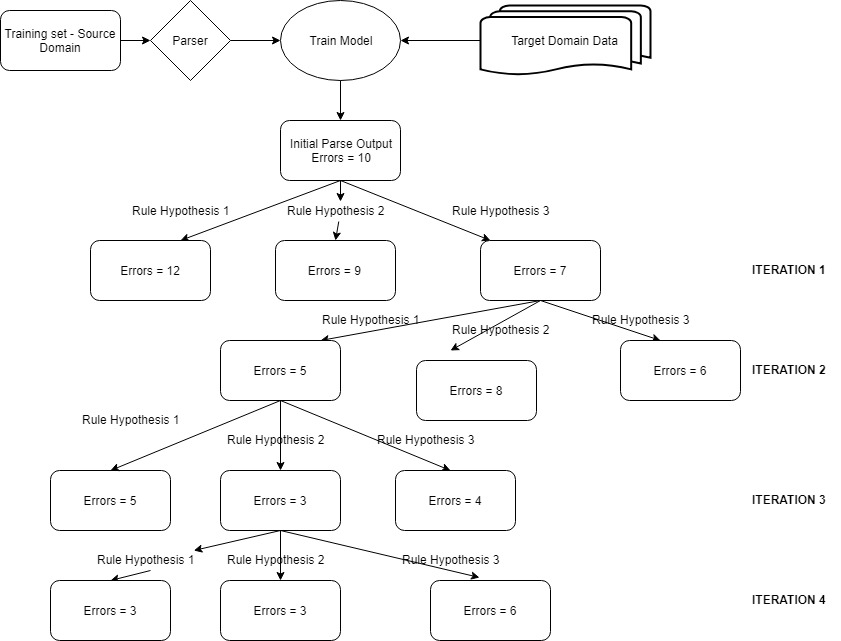
\includegraphics[scale = 0.34]{tbedl.png}
    \centering
    \caption{Reducing dependency label errors via transformation-based error-driven learning\textcolor{white}{try this}}
    \label{fig:tbedl}
\end{figure*}

\textcolor{white}{try this}

\begin{algorithm}[!t]
 \caption{TBL for Domain Adaptation}\label{alg:tbl}
\begin{algorithmic}[1]
\Procedure{$TBL\_learn$}{$training\_data$}
\State $work\_copy\ =\ extract\ text\ from\ training\_data;\ parse\ using\ WSJ\ model$
\State $learned\_rules \gets []$
\Repeat
\LineComment{Generate rule hypothesis from errors in corpus given rule templates}
\State $rule\_hypotheses = generate\_hypotheses(training\_data,work\_copy)$ 
%\vspace{.2em}
\LineComment{calculate improvement score for each rule:  \# errors fixed}
\State $rule\_scores = determine\_scores(rule\_hypotheses, work\_copy)$ 
%\vspace{.1em}
\LineComment{Rank rules given scores; select rule with highest score}
\State $best\_rule, best\_score = argmax(rank\_rules(rule\_hypotheses, rule\_scores)$
%\vspace{.2em}

\LineComment{If best rule causes improvement, apply rule to work copy}
\If{$best\_score > 0$}
\State $work\_copy = apply\_rule(work\_copy, best\_rule)$
\State $learned\_rules \mathrel{+}= best\_rule$
\EndIf
%\LineComment{In the next iteration, we use this changed training data and repeat the process until the number of errors are not reduced anymore.}
\vspace{-1em}
\State \Until{$best\_score <= 0$}
\State \textbf{return} $learned\_rules$
\EndProcedure
\vspace{1em}
\Procedure{$TBL\_apply$}{$learned\_rules, test$}

\State $test\_annotated\ =\  parse\ test\ data\ using\ WSJ\ model$
\LineComment{Apply learned rules in order to test set}
\For{each rule in learned\_rules}
\State $test\_annotated = apply\_rule(test\_annotated, rule)$

\EndFor
\EndProcedure


\end{algorithmic}

\end{algorithm}


We outline the process in algorithm~\ref{alg:tbl}. The learning iterates until there are no more rule hypotheses that would cause a further reduction in errors. During each iteration, based on the templates, the algorithm creates rule hypotheses from the errors found by comparing the working copy to the gold standard. It then chooses the best rule hypothesis that maximally reduces the errors in the working copy and applies this rule to the working copy. %We measure the improvement for each of the rule hypothesis and return the hypothesis (1 or multiple) with most improvement in terms of errors. 
Since the templates that we use are independent of each other, we currently apply the top 10 rules per iteration. Choosing to apply multiple rules speeds up the overall process. To prevent over-generation, we favor the more specific hypothesis if there is a tie in the scores. We then store these rules in the final list of learned rules. %However, our process is flexible enough, such that, this threshold could be changed to any integer.
After the application of the rules chosen in each iteration, we use the updated work copy in the next iteration. %The process finishes when there is no more change in the number of errors. 

After learning, a new text is processed by first having it parsed by the source domain dependency parser and then applying the learned rules in order.

% We instantiate these rule templates on the gold standard corpus and obtain a set of possible rule hypotheses. We do the following iteratively:
% \begin{enumerate}
%     \item We apply the rule hypotheses on the initial state corpus.
%     \item We calculate the reduction in error for each of these rule hypotheses.
%     \item We keep track of the rule hypotheses with the highest improvement in terms of reduction of errors at each iteration. We calculate improvement score($S_i$) as:
%     $$S_i = e_{prev} - e_{curr}$$
%     where $e_{prev}$ is the error prior to applying the rule hypothesis and $e_{curr}$ is the number of errors after applying the rule hypothesis.
%     Since, we do not use dependency labels as variables for our templates, instead of applying the one rule per iteration, we can apply more. For this paper, we choose a threshold of 10. 
%     \item We add these rules with the highest improvement scores to the list of final learned rules.
%     \item We continue until we get no further reduction in errors.
% \end{enumerate}

%After, we get the final list of learned rules from this process, the next step is to apply these rules to the test set. %We evaluate the system by measuring the Labeled Attachment Score (LAS-1) and Labeled Accuracy Scores (LAS-2).

\section{Experimental Setting} \label{sec:exptsetup}

%We report experiments using the following two domains: financial news articles  (WSJ)~\cite{Marcus:1994:PTA:1075812.1075835} and dialogues recorded during a collaborative task (CReST)~\cite{eberhard2010indiana}.  WSJ serves as our source domain, thus we create a parsing model using MATE parser~\cite{bohnet:2010:PAPERS,bohnet2010very}. We parse sentences from CReST using this model. Since the source domain (WSJ) and the target domain (CReST) have differences in dependency label annotation, this introduces some errors in the resulting parse. 

\subsection{Data Sets}
In our current work, we focus on two domains: financial news articles and dialogues in a collaborative task.
We use the Wall Street Journal \cite{Marcus:1994:PTA:1075812.1075835} and the CReST corpus~\cite{eberhard2010indiana} as representative corpora for these two domains. %Wall Street Journal consists of financial articles, news, etc. CReST corpus, on the other hand, comprises of dialogues recorded during a collaborative task.%natural language dialogues between two people, who carry out a certain task with the help of each other. 
%%SK check numbers? - x

These corpora are very dissimilar in nature. On  average, the length of the sentences for WSJ is 24 and 7 for CReST. In terms of linguistic factors, CReST has a subset of WSJ's dependency labels with 10 new labels added.%and 
%%SK why do we care about POS tags? should that be dep labels? - atr: because I was thinking this might also show how different the corpora are, but its not needed.
%has 14 different part of speech tags than WSJ. 
Example sentences from each corpora are shown in table~\ref{tab:samplesentences}. We use WSJ as the source domain and CReST as the target domain.  %We create a parsing model using the MATE parser~\cite{bohnet:2010:PAPERS,bohnet2010very}. We then parse sentences from CReST using this model. %Since the source domain (WSJ) and the target domain (CReST) have differences in dependency label annotation, this introduces some errors in the resulting parse. 

\begin{table}[!t]
\centering
\begin{tabular}{l|l}
\hline
WSJ   & \begin{tabular}[c]{@{}l@{}}
In an Oct. 19 review of " The Misanthrope " at Chicago 's Goodman Theatre \\ ( " Revitalized Classics Take the Stage in Windy City , " Leisure \& Arts ) , \\ the role of Celimene , played by Kim Cattrall , was mistakenly attributed \\ to Christina Haag .\end{tabular} \\ \hline
CReST & \begin{tabular}[c]{@{}l@{}}
it's like as soon - like if I were to close the door it's right next to like the \\ bottom of the floor like where the door closes 
\end{tabular} \\ \hline
%so I went through some - I went through the second room right? \\ \hline    
%can I tell you where that is?   
\end{tabular}
\caption{Sample sentences from Wall Street Journal (WSJ) \& CReST corpus}
\label{tab:samplesentences}
\end{table}



\paragraph{Target Domain}
The CReST corpus consists of 23 dialogues that were manually annotated for dependencies. We randomly select 19 dialogues as our training data and the rest as test. 
since the system needs to learn rule hypotheses from  incorrect predictions of the source domain parser, 
we can safely ignore sentences that were parser completely correctly. For the test data, we use all the sentences from the designated dialogues (with correct and incorrect dependency label predictions). 
%As a part the training part of Transformation Based Error Driven Learning (TBL), the system needs to learn rule hypotheses from the incorrect dependency label prediction, we work on the sentences which show errors in dependency labels. 
Table~\ref{tab:sentdiv} shows the division of sentences for training and test.

\begin{table}[t]
\centering
\begin{tabular}{l|l|c|c}
& \multirow{2}{*}{\# Dialogues} & \multicolumn{2}{c}{\# Sentences} \\ \cline{3-4}
 &  & \multicolumn{1}{l|}{with errors} & \multicolumn{1}{l}{without errors} \\ \hline
Training Set & \multicolumn{1}{|c|}{19} & 4384 & 459 \\
Test Set & \multicolumn{1}{|c|}{4} & 831 & 85 \\ \hline
\end{tabular}
\caption{Target domain training and test set for TBL}
\label{tab:sentdiv}
\end{table}

% \begin{enumerate}[label=Setting \arabic*,leftmargin=*]
% %\setlength\itemsep{2pt}
%     \item We consider all the sentences set aside as the test set has incorrect dependency labels.
%     \item Test set contains a mix of sentences with correct and incorrect dependency labels. 
% \end{enumerate}

\subsection{TBL Components}

\paragraph{Initial State System}
We use the MATE parser~\cite{bohnet:2010:PAPERS} as the initial state annotator. We use 17~181 sentences from WSJ to train the MATE parser. We use this model to parse the sentences from the CReST training set to obtain the initial state annotated text.

\paragraph{Baseline}

We benchmark our results against the performance of the MATE parser trained on WSJ sentences, i.e., the out-of-domain parser, without any modification. We also report results for an in-domain setting where the MATE parser is trained on the CReST training set.


\subsection{Evaluation}
For evaluation, we use the CoNLL-X script. We report the Labeled Attachment Scores  (LAS) and Label Accuracy  (LA) as the primary metrics for evaluating our system. LAS measures the percentage of words which have the correct head and dependency label. LA measures the number of correctly assigned labels. Reporting LA is important  since this measure focuses solely on the accuracy of the labels while LAS also evaluates structural issues in the parse, which we do not address currently. We
also report the exact syntactic match (EM), which measures the percentage of sentences that have correct overall predicted dependency trees.

\section{Experimental Results} \label{expt_results}

In this section, we discuss the outcome of our experiments for the TBL process. The results of applying the rules learned from TBL are given in table~\ref{tab:overall}.
%4 rule templates
%improv>1 -> deprel = 471
%   Labeled   attachment score: 4079 / 5823 * 100 = 70.05 %
%   Unlabeled attachment score: 4308 / 5823 * 100 = 73.98 %
%   Label accuracy score:       5352 / 5823 * 100 = 91.91 %
%2 rule templates
%improv>1 -> deprel = 660
%  SYNTACTIC SCORES:
%   Labeled   attachment score: 4053 / 5823 * 100 = 69.60 %
%   Unlabeled attachment score: 4308 / 5823 * 100 = 73.98 %
%   Label accuracy score:       5163 / 5823 * 100 = 88.67 %
%   Exact syntactic match:      438 / 916 * 100 = 47.82 %
%%SK what does 'WSJ-modeled output' mean? baseline? -x


\begin{table}[t]
\centering
%\resizebox{\textwidth}{!}{%   
\begin{tabular}{l|l|r|rrr|}
 & \multicolumn{1}{c|}{Setting} & \# Incorrect  & LAS & LA & EM \\ \hline
1 & Baseline (trained on WSJ) & 2~112 & 59.02  & 63.73 & 8.41  \\
%2 & In-domain baseline (trained on CReST)& 1~289 & \textbf{72.57}  & 77.86 & \textbf{53.49}   \\
2 & In-domain baseline (trained on CReST)& 572 & \textbf{87.39}  & 90.18 & \textbf{67.58}   \\
3 & Rule Templates (1+2) & 600 & 69.91  & 89.70 & 48.03 \\
4 & Rule Templates (1+2+3+4) & {451} &{\textbf{\textit{70.10}}} &
{\textbf{92.25}} & {\textbf{\textit{48.80}}}  \\
%1 & Baseline (WSJ-parsed output) & 2~112 & 59.02  & 63.73 & 8.41  \\
\hline
\end{tabular}%
%}
\caption{Results of applying TBL rules on test set.}
\label{tab:overall}
\end{table}


The first setting is our baseline. We evaluate the performance of our system against the results of parsing the sentences from the test set with the model trained on WSJ. The second baseline consists of an in-domain parser trained on the small CReST training set. Settings 3 and 4 evaluate the performance of the learned rules. The third setting derives rule hypotheses instantiated by 2 rule templates (rule templates 1 \& 2). Since rule templates 1 \& 2 are more specific (it accounts for lemma as well as part of speech tags), we add more general templates such as POS tags specifically (rule templates 3 \& 4) to investigate if that leads to a significant difference in the results. %We also report the in-domain results as setting 4.%Thus, this setting evaluates the results of applying rules learned from 4 rule templates (rule templates 1, 2, 3 and 4). We include the results of in-domain parsing as setting 4.
%%SK OK, can we also mention what the 2 and 4 templates are? Did you adjust the numbers in the table after you sorted the templates in sec. 4.2? And can you tell us why these two settings? - x

From table~\ref{tab:overall}, we observe that applying TBL has a significant effect on the quality of the predicted dependency labels, with an improvement in LAS of almost 20\% absolute over the out-of-domain parses. The number of completely correct sentences shows an improvement of 40\% absolute over this baseline. We also see that extending the set of templates to include less-specific templates (templates 3 and 4) using POS tags information, has a minimal effect on LAS but increases label accuracy (LA) by 2.5\% absolute. 

\begin{table}[t]
\centering
\begin{tabular}{l|r|rrr|}
\multicolumn{1}{c|}{\multirow{2}{*}{Label}} & \multirow{2}{*}{\# in Gold} & \multicolumn{3}{c|}{\% Correct} \\ \cline{3-5}
\multicolumn{1}{c|}{} &  & baseline &2 templates & 4 templates \\ \hline
INTJ & 690 & 0 & 98.26 & 99.71 \\
ROOT* & 195 & 0 & 63.59 & 77.44 \\ \hline
%VMOD & 1 & 0 & 0 & 0 \\ \hline
\end{tabular}
\caption{Accuracy in predicting CReST-specific labels.}
\label{tab:labelcomp}
\end{table}



%When comparing the TBL results  to the in-domain baseline, we notice that the baseline reaches an LAS that is about 2.5\% higher than the TBL results, but the TBL approach reaches considerably higher results with regard to LA (92.25\% vs.\ 77.86\%). The different trends can be explained by the fact that we are currently restricting the TBL approach to functional changes, and we ignore structural errors. Since the LAS evaluates both aspects, we see that the in-domain parser fares better in this respect. However, the LA, which only evaluates dependency labels, shows that our method is very successful in improving the labels. 

When comparing the TBL results  to the in-domain baseline, we notice that the baseline reaches an LAS considerably higher than the TBL results, but the TBL approach using all 4 templates reaches higher results with regard to LA (around 2\% improvement). The different trends can be explained by the fact that we are currently restricting the TBL approach to functional changes, and we ignore structural errors. Since LAS evaluates both aspects, we see that the in-domain parser fares better in this respect. However, the LA, which only evaluates dependency labels, shows that our method is successful in improving the labels. Since the results of the experiment with 2 templates are similar to the in-domain treebank, we assume that we need to experiment with more specific templates in the future.


%Since we do not revise dependency heads, the unlabeled attachment score remains the same at 73.98\% for settings 1,2 \&3 but increases to 77.13\% for setting 4. This leads to a higher LAS than the TBL setting. However, LA is significantly higher for the TBL setting  with more than 14\% improvement which shows the effectiveness of applying TBL to reduce the number of incorrect dependency labels. The results will be comparable when we add structural transformations (i.e., correcting dependency heads) in our TBL settings.
%Although LAS is higher in in-domain setting - owing to the improved UAS - than setting 3, LA is significantly higher for the TBL setting. (14.39\% improvement; with more than 50\% improvement in reducing label confusions). 
%%SK please add -x 

There are 10 dependency labels in CReST which do not occur in WSJ. Out of these, 2 labels  (ROOT\textsc{*}, INTJ) occur in the test data. ROOT\textsc{*} is used for words whose head is missing because the sentence was interrupted; and INTJ is used for interjections. Since WSJ does not use these labels, these are predicted incorrectly in all the cases in the out-of-domain baseline. 

We investigate the number of times these labels have been corrected by TBL. Table~\ref{tab:labelcomp} shows the results. As expected, the labels do not show up in the baseline setting. For the settings using 2 or 4 templates, there is a significant improvement for the labels INTJ and ROOT\textsc{*}. 
%%SK I think that is an annotation error? - x
% However, the label VMOD has not been predicted accurately (predicted as ADV). We examine the training set for contextual information on the label. % atr - I don't know how to write this
% For the same context (parent/dependents/lemma), the label ADV appears 54 times whereas the label VMOD appears once. 


\begin{table}[t]
\resizebox{\textwidth}{!}{%

\begin{tabular}{ccccccccc} 
\hline
Rule Template & Lemma (self) & Pos (self) & Lemma (head) & POS (head) & Lemma (children) & POS (children) & Deprel & Improvement \\ \hline
RT2 & okay & UH & (root word) & (root word) & - & - & INTJ & 1292 \\
RT2 & um & UH & (root word) & (root word) & - & - & INTJ & 386 \\
RT2 & be & VBZ & (root word) & (root word) & - & - & ROOT & 384 \\
RT2 & alright & UH & (root word) & (root word) & - & - & INTJ & 216 \\
RT2 & yeah & UH & (root word) & (root word) & - & - & INTJ & 205 \\
RT2 & the & DT & (root word) & (root word) & - & - & ROOT* & 131 \\
RT3 & and & CC & be & VBZ & (no children) & (no children) & COORD & 117 \\
RT2 & go & VBI & (root word) & (root word) & - & - & ROOT & 100 \\
RT3 & that & DDT & be & VBZ & (no children) & (no children) & SBJ & 83 \\
RT2 & well & UH & (root word) & (root word) & - & - & INTJ & 77 \\ \hline
\end{tabular}%
}
\caption{Top learned rules for the setting using 2 templates.}
\label{tab:2templatestoprules}
\end{table}

Table~\ref{tab:2templatestoprules} and \ref{tab:4templatestoprules} show  the 10 learned rules with the highest scores, for the setting with 2 or 4 templates respectively. We can observe that many of the rules concern the labels INTJ and ROOT\textsc{*}. Since these labels do not appear in the source domain, applying rule hypotheses specific to these labels leads to the highest gains. 

To have a closer look, we extracted the most frequent label confusions for each setting after parsing and TBL domain adaptation. The results are shown in table~\ref{tab:depconf}. For the baseline, the most frequently incorrect label is INTJ, followed by ROOT and ROOT\textsc{*}. By applying TBL, we have countered the most frequent label confusion as evident from the settings using 2 or 4 templates, where the numbers are lower across the board, but also the types of confusion are more typical of standard parsing issues (e.g., subject (SBJ) vs.\ predicate (PRD)).


\begin{table}[t]
\centering
\resizebox{\textwidth}{!}{%
\begin{tabular}{ccccccccc}
\\ \hline
Rule Template & Lemma (self) & POS (self) & Lemma (head) & POS (head) & Lemma (children) & POS (children) & Deprel & Improvement \\ \hline
RT4 & - & UH & - & (root word) & - & - & INTJ & 2886 \\
RT5 & - & UH & - & (root word) & - & (no children) & INTJ & 2766 \\
RT2 & okay & UH & (root word) & (root word) & - & - & INTJ & 1292 \\
RT3 & okay & UH & (root word) & (root word) & (no children) & (no children) & INTJ & 1271 \\
RT4 & - & AP & - & (root word) & - & - & INTJ & 453 \\
RT5 & - & AP & - & (root word) & - & (no children) & INTJ & 438 \\
RT2 & um & UH & (root word) & (root word) & - & - & INTJ & 386 \\
RT2 & be & VBZ & (root word) & (root word) & - & - & ROOT & 384 \\
RT3 & um & UH & (root word) & (root word) & (no children) & (no children) & INTJ & 383 \\
RT5 &  & XY &  & (root word) &  & (no children) & ROOT* & 268 \\ \hline
\end{tabular}%
}
\caption{Top learned rules for the setting using 4 templates.}
\label{tab:4templatestoprules}
\end{table}



% \begin{table}[!htb]
% \centering
% \begin{tabular}{c|c|c|c}
% \multicolumn{2}{c|}{Setting - 2} & \multicolumn{2}{c}{Setting - 3} \\ \hline
% Best Rule Template & Improvement & Best Rule Template & Improvement \\ \hline
% RT2 & 1292 & RT4 & 2886 \\
% RT2 & 386 & RT5 & 2766 \\
% RT2 & 384 & RT2 & 1292 \\
% RT2 & 216 & RT3 & 1271 \\
% RT2 & 205 & RT4 & 453 \\
% RT2 & 131 & RT5 & 438 \\
% RT3 & 117 & RT2 & 386 \\
% RT2 & 100 & RT2 & 384 \\
% RT3 & 83 & RT3 & 383 \\
% RT2 & 77 & RT5 & 268 \\ \hline
% \end{tabular}
% \caption{Top 10 rules learned by the system}
% \label{tab:bestrules}
% \end{table}


% \begin{table}[]
% \centering
% \resizebox{\textwidth}{!}{%
% \begin{tabular}{llcccccccccccccccc}
%  &  & \multicolumn{7}{c}{Setting - 2} & \multicolumn{9}{c}{Setting - 3} \\
% Rule Template & Lemma (self) & Pos-self & Lemma (head) & POS (head) & Lemma (children) & POS (children) & Deprel & Improvement & Rule Template & Lemma (self) & POS (self) & Lemma (head) & POS (head) & Lemma (children) & POS (children) & Deprel & Improvement \\
% RT2 & okay & UH & (root word) & (root word) & - & - & INTJ & 1292 & RT4 & - & UH & - & (root word) & - & - & INTJ & 2886 \\
% RT2 & um & UH & (root word) & (root word) & - & - & INTJ & 386 & RT5 & - & UH & - & (root word) & - & (no children) & INTJ & 2766 \\
% RT2 & be & VBZ & (root word) & (root word) & - & - & ROOT & 384 & RT2 & okay & UH & (root word) & (root word) & - & - & INTJ & 1292 \\
% RT2 & alright & UH & (root word) & (root word) & - & - & INTJ & 216 & RT3 & okay & UH & (root word) & (root word) & (no children) & (no children) & INTJ & 1271 \\
% RT2 & yeah & UH & (root word) & (root word) & - & - & INTJ & 205 & RT4 & - & AP & - & (root word) & - & - & INTJ & 453 \\
% RT2 & the & DT & (root word) & (root word) & - & - & ROOT* & 131 & RT5 & - & AP & - & (root word) & - & (no children) & INTJ & 438 \\
% RT3 & and & CC & be & VBZ & (no children) & (no children) & COORD & 117 & RT2 & um & UH & (root word) & (root word) & - & - & INTJ & 386 \\
% RT2 & go & VBI & (root word) & (root word) & - & - & ROOT & 100 & RT2 & be & VBZ & (root word) & (root word) & - & - & ROOT & 384 \\
% RT3 & that & DDT & be & VBZ & (no children) & (no children) & SBJ & 83 & RT3 & um & UH & (root word) & (root word) & (no children) & (no children) & INTJ & 383 \\
% RT2 & well & UH & (root word) & (root word) & - & - & INTJ & 77 & RT5 &  & XY &  & (root word) &  & (no children) & ROOT* & 268
% \end{tabular}%
% }
% \end{table}


% \begin{table}[!t]
% \centering
% \resizebox{\textwidth}{!}{%
% \begin{tabular}{ccc|ccc|ccc|ccc}
% \multicolumn{3}{c|}{Setting 1} & \multicolumn{3}{c|}{Setting 2} & \multicolumn{3}{c|}{Setting 3} & \multicolumn{3}{c}{Setting 4} \\ \hline
% Gold & Predicted & Counts & Gold & Predicted & Counts & Gold & Predicted & Counts & \multicolumn{1}{c}{Gold} & \multicolumn{1}{c}{Predicted} & \multicolumn{1}{c}{Counts} \\ \hline
% INTJ & ROOT & 354 & ROOT* & ROOT & 39 & ROOT* & ROOT & 38 & 57 & ROOT & NMOD \\
% INTJ & DEP & 210 & SBJ & PRD & 20 & SBJ & PRD & 25 & 47 & LOC & ROOT \\
% ROOT & NMOD & 136 & ROOT* & NMOD & 20 & ROOT & ROOT* & 21 & 36 & NMOD & ROOT \\
% ROOT* & NMOD & 100 & LOC & NMOD & 19 & DIR & LOC & 19 & 33 & ROOT* & NMOD \\
% INTJ & NMOD & 85 & ROOT & ROOT* & 17 & DIR & ADV & 17 & 27 & LOC & DIR \\
% LOC & NMOD & 55 & DIR & ADV & 15 & LOC & NMOD & 15 & 25 & ROOT* & ROOT \\
% COORD & DEP & 38 & ROOT & NMOD & 13 & TMP & ADV & 10 & 23 & VC & NMOD \\
% ROOT & COORD & 37 & DIR & NMOD & 12 & LOC & ADV & 10 & 22 & SBJ & NMOD \\
% LOC & LOC-PRD & 35 & LOC & ADV & 11 & ROOT & NMOD & 8 & 21 & P & NMOD \\
% LOC & PRD & 33 & PMOD & NMOD & 10 & OBJ & SBJ & 8 & 20 & NMOD & PRD \\ \hline
% \end{tabular}%
% }
% \caption{The 10 most frequent label confusions across the different settings.}
% \label{tab:depconf}
% \end{table}


\begin{table}[!t]
\centering
\resizebox{\textwidth}{!}{%
\begin{tabular}{ccc|ccc|ccc}
\multicolumn{3}{c|}{Baseline} & \multicolumn{3}{c|}{2 Templates} & \multicolumn{3}{c}{4 Templates} \\ \hline
Gold & Predicted & Counts & Gold & Predicted & Counts & Gold & Predicted & Counts \\ \hline
INTJ & ROOT & 354 & ROOT* & ROOT & 39 & ROOT* & ROOT & 38 \\
INTJ & DEP & 210 & SBJ & PRD & 20 & SBJ & PRD & 25 \\
ROOT & NMOD & 136 & ROOT* & NMOD & 20 & ROOT & ROOT* & 21 \\
ROOT* & NMOD & 100 & LOC & NMOD & 19 & DIR & LOC & 19 \\
INTJ & NMOD & 85 & ROOT & ROOT* & 17 & DIR & ADV & 17 \\
LOC & NMOD & 55 & DIR & ADV & 15 & LOC & NMOD & 15 \\
COORD & DEP & 38 & ROOT & NMOD & 13 & TMP & ADV & 10 \\
ROOT & COORD & 37 & DIR & NMOD & 12 & LOC & ADV & 10 \\
LOC & LOC-PRD & 35 & LOC & ADV & 11 & ROOT & NMOD & 8 \\
LOC & PRD & 33 & PMOD & NMOD & 10 & OBJ & SBJ & 8 \\ \hline
\end{tabular}%
}
\caption{The 10 most frequent label confusions across the different settings.}
\label{tab:depconf}
\end{table}


%\clearpage
\section{Discussion} \label{conclusion}
% x

In this paper, we introduce transformation-based error-driven learning (TBL) for domain adaptation in dependency parsing. Since there tend to be significant differences between annotation schemes of different corpora from different domains, we focus on methods that can address those differences systematically along with differences due to the domain itself.  When a text is parsed with a model trained on one domain, it leads to a significant number of incorrect predictions, especially for dependency labels. %This is because source and target might have different labels. As we show in our analysis, this is indeed the case. 
We address this problem in our work by using TBL to learn rules from a small target domain training set and a small set of manually defined rule templates. % by iteratively applying rule hypotheses and learning the rules with the best improvement. 
In comparison to a pure out-of-domain parser, we observe a significant increase in the labeled attachment scores (\char`\~20\%), labeled accuracy (\char`\~30\%) and exact match (\char`\~40\%) for WSJ as source and CReST as target corpus. The observed improvement is largely due to the labels that are used in CReST, but do not occur in WSJ since those are mislabeled consistently by the out-of-domain parser. However, when we apply TBL, these labels are corrected in most of the cases. When we compare our results to an in-domain parser, the results show that the TBL approach is very
 good at correcting the dependency labels, but we need to extend the approach and use more specific templates and cover structural errors as well to be able to compete with the in-domain parser with regard to LAS. 

Our method is flexible in that any number of variables can be used in the templates, and it can be extended to cover structural changes, i.e., to correct dependency head annotations. In addition, the templates are valid across different target domains.

As a part of our future work, we plan to evaluate the effectiveness of this method for multiple domains. We will also introduce new variables in our rule templates including contextual information on dependency labels. In addition to correcting dependency labels, we will extend the method to correct predicted dependency heads by introducing new templates. This will need to be accompanied by a check to ensure that the resulting analysis is still a valid dependency graph. 
